\documentclass[../main/Feedback.tex]{subfiles}
\begin{document}
\section{Experiment Design}
We used fNIRS because it is non-invasive, have low sensitivity to motion artefacts, and with high temporal resolution, thus suitable for user trials. We combine the fNIRS, as an objective measure of mental workload with the subjective NASA-TLX as they are validated and reliable methods. In addition, we decided to measure the emotional valence with the SAM questionnaire. This way we gather comprehensive information about how participants perceive the interfaces and relate it to the psychophysiological data. Furthermore, fNIRS is novel method for conducting usability studies, and as such we aim to assess its practicality.

\subsection{Participants}
A total of 20 right handed participants (9 female) with mean age of 26 (SD = 4.04) took part in the study. All of the participant were healthy, however only one pointed that it suffers ``Von Willebraud disease'' which impairs blood's ability to clot, and his data from the psychophysiological measures was excluded. All participants had normal or corrected to normal vision, and report no history of brain damage. Also, 14 of them reported they have advanced computer literacy, 5 of them stated average computer literacy and 1 did not answer this question. All of the participants were current or graduated students. The ethics committee of the University of Nottingham approved this study. Informed consent was obtained from the participants and they were compensated with £10 Amazon voucher.
\subsection{Apparatus}
\subsubsection{Laptop computer}
The experiment was executed on 15" laptop, HP probook 450 with screen resolution 1366x768. An external mouse was attached, which participants used during the process. The participant was presented with a screen with links to the three different videos and web forms. They were instructed by the researcher to manually start certain condition or video. 
\subsubsection{fNIRS}
Hemodynamic data was recorded using the fNIRS300 device along with the COBI studio recording software developed by Biopac Systems inc. The device consists of a headband with 4 infrared LED emitters and 10 infrared detectors as it can be seen from Figure \ref{fig:source-detector-diagram}. 				
\begin{figure}[h]
	\centering
	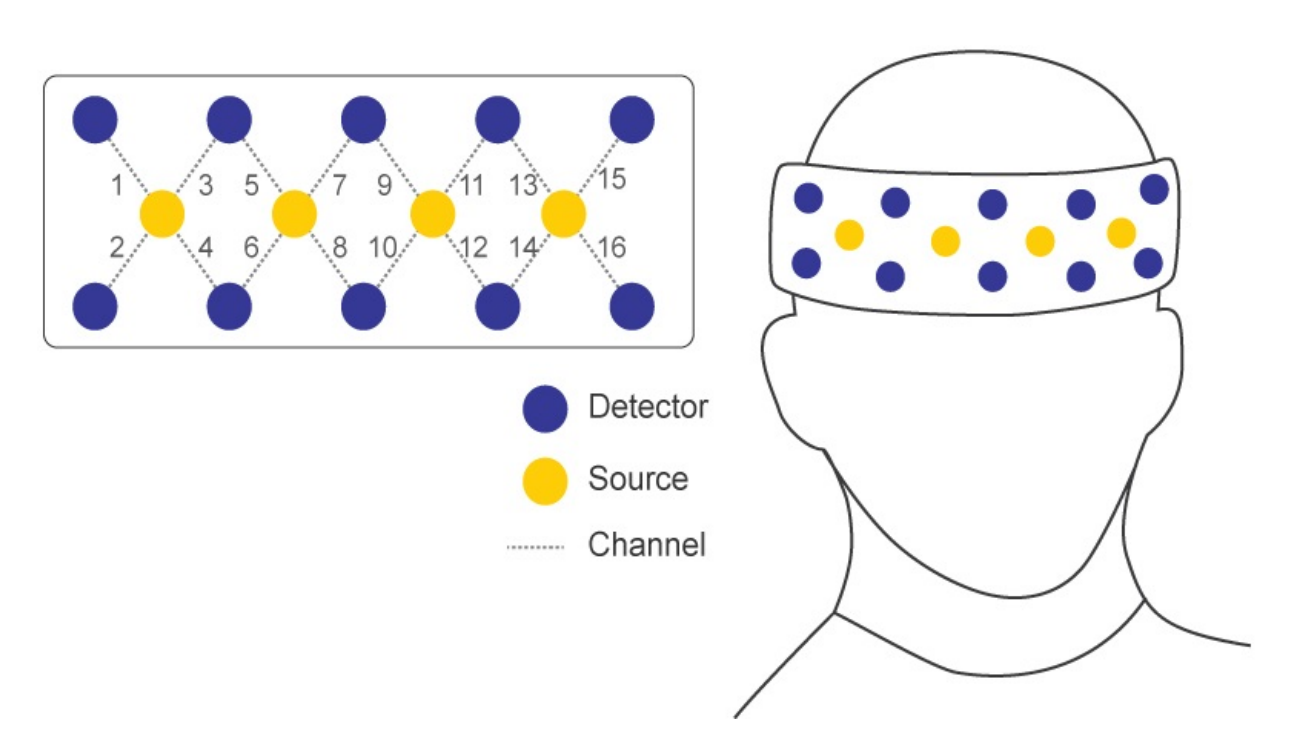
\includegraphics[width=0.7\linewidth]{source-detector-diagram}
	\caption[fNIRS source-detector diagram]{The spatial arrangement of the source-detector pars placed on participants forehead.}
	\label{fig:source-detector-diagram}
\end{figure}
They operated on 730nm and 850nm wavelengths. The combination between them was used to calculate 16 channels which can measure the associated Hbo and Hbr concentration in the PFC. The fNIRS device was placed on the forehead of the participants targeting the dorsolateral(BA 9/46) and orbitofrontal(BA 10) cortices.
\subsection{Materials}
\subsubsection{NASA-TLX}
The NASA-TLX\cite{nasatlx} is multidimensional subjective scale and it is used as a tool for assessing operator workload based weighted average of its six scales. The individual scales are presented in the following order: Mental demand, Physical demand, Temporal demand, Performance, Effort, and Frustration. We used the paper version of the questionnaire. The NASA-TLX measures were obtained from participants each time after completing one of the web form conditions. We did not follow the weighting procedure because it was time consuming, and instead we calculated the mean values of all individual subscales, which is suggested to be also, a valid measure\cite{hart2006nasa}, and we refer to this variable as ``total tlx''. Furthermore, each of the individual subscales was analysed independently.
\subsubsection{Self assessment manikin scale (SAM)}
Self assessment manikin\cite{bradley1994measuring} is a two dimensional scale for measuring the perceived emotional valence and arousal. We implemented the 5 point version of it. The participants were asked to fill the questionnaire after each video watched and each web form filled. First they state their emotional valence(negative or positive) by choosing between 1 and 5, where 5 is strongly perceived positive emotion, and 1 is considered strong negative emotion. Then, they fill the arousal level scale, where 1 indicates low perceived arousal or boredom, and 5 signifies high perceived arousal or high level of excitement. Each of the subscales is supported by image visualisations illustrating the affective state.
\subsubsection{Layout variations of web forms}
\begin{figure}
	\centering
	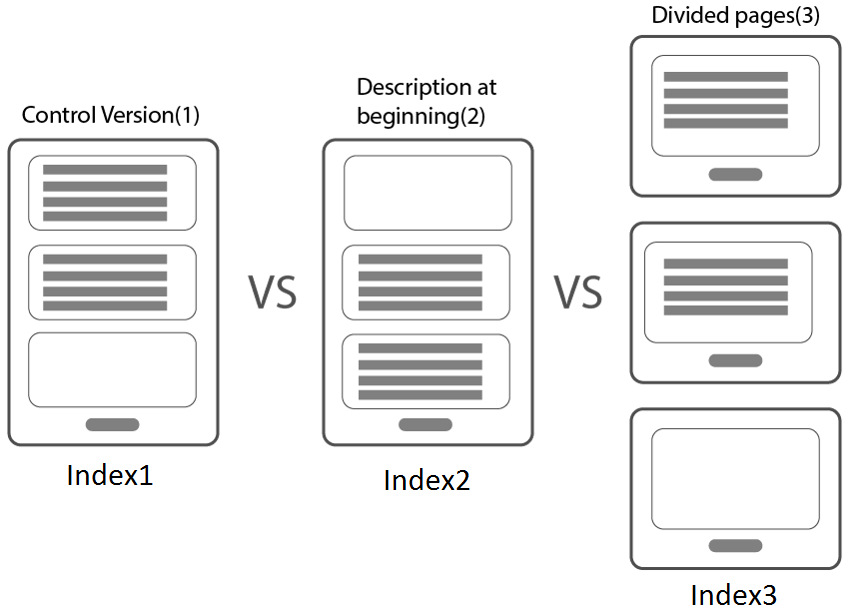
\includegraphics[width=0.86\linewidth]{layout-variations}
	\caption[Sketch of layout variations of the web forms]{A sketch of the 3 layout variations of the web forms. The control condition index1 asked first for personal information, then accident information, and finally asks for description of the accident. With Index2 the description field was placed at the beginning. Index3 had 3 sections separated on 3 sequential pages.}
	\label{fig:layout-variations}
\end{figure}
A total of 3 HTML/CSS variations of a standard web form for insurance claiming were produced. A generalized sketch is depicted in Figure \ref{fig:layout-variations}. They were created to resemble an actual online insurance claim form. All of the conditions were divided on 3 main divisions: Personal information, Accident information and Summary of accident. The personal information division consisted of 5 individual forms, namely: First name, Last name, Date of birth, Email, You are(choose type of stakeholder, which was option field). The accident information consisted of one text input field(Today's date), four drop down lists(Number of passengers, Number of cars involved in the accident, Was anyone injured in this incident, and Was the accident caused by your fault), and a checkbox form for selecting which areas of the vehicle were damaged. Lastly, the third division consisted of a text-area, where participants had to write a description of the accident. The first version or the control version, referred as index1, consisted of the 3 division areas laid out in the order that was described here, namely, at the top of the page is the personal information, followed by accident information and lastly summary of accident. In the second web form, which we refer to as index2, the summary of accident area was placed on the top of the page, followed by personal and accident information, accordingly. The third condition, referred as index 3 had the same order as index1, however each division area was situated on separate page, and consisted of total 3 pages. Users navigated between the three pages using a submit button with the label``Next''. Also, on the top of the form below the heading there was a progress feedback text indicating of how many steps the web form consisted. For more detailed information, the three web form conditions can be viewed in the attached zip file, that contains all the data.
\subsubsection{Video capture}
A video capture of the computer screen was recorded during the experiment using Fraps\cite{fraps}. The participants voice was recorded too. The timestamp of the beginning of the video recording was obtained, in order to be able to calculate duration of tasks, and their actual start and end time.
\subsubsection{Video clips of auto accidents}
Three video clips of automotive accidents were selected, in order to simulate the conditions before the filling of insurance claim. The video clips of the accidents were chosen to be lightweight avoiding any scenes of gore, injured bodies, or fatalities. All of the accidents happened in low speed. One of the clips has a duration of minute and a half, while the others were half a minute long. The three videos can be seen in the attached zip file.
\subsection{Design}
The study used repeated measures within subjects design. The depended variable was the mental workload, and the independent variable was the layout of the three web forms. The control condition was index1. Before the start of each web form, a video of road accident was played. The three variations of videos and the web forms were counterbalanced using Latin square rotation, in order to avoid learning effects from the order of presentation of the video clips.
\subsection{Procedure}
\begin{figure}[h]
	\centering
	\includegraphics[width=0.95\linewidth]{"study-procedure"}
	\caption[study procedure]{The image illustrates, the study procedure followed in this experiment. First participants, watched video, then fill the SAM measure. After that, they filled the a web form, and then filled both the NASA-TLX and SAM scales. The process was repeated 3 times.}
	\label{fig:study-procedure}
\end{figure}		
Participants followed the procedure illustrated by Figure\ref{fig:study-procedure}. First, participants were asked to read and sign information sheet and consent forms. Second, the fNIRS device was cleaned then equipped and started. Third, participants were briefed about the procedure of the experiment, and it was explained how to fill the subjective scales. Also, because of ethical considerations that the participant should not enter personal data in the web form, a artificial personal credentials were provided, that she should fill in the web forms. Fourth, after the video capture and the fNIRS device were started, participants were asked to relax and try not to think about anything, in order to record a baseline of the hemodynamic activity in the PFC while participants are at rest. Next, they are asked to open one of the three videos, depending on the counterbalancing table. After the video was finished, participants fill SAM subjective scale. Fifth, there was approximately 2 minute waiting period between the video and the web form filling task, so that participant's memory is not fresh. Finally, after participant has completed the web form, the SAM and then the NASA-TLX scales are given to be completed, accordingly. This process was repeated three times, following the within subjects experimental design with counter balancing between the videos and the web forms. Because fNIRS device used one computer and the experiment was conducted on different computer, before each experiment, the clocks between the two computers were synchronized. Also, timestamps using the Cobi Studio software manual markers were created in the beginning and end of each condition and video. 
\subsection{Data Analysis}
The fNIRS data was analysed with fnirsoft\cite{ayazfunctional}. Data from N=1 participant was excluded from the analysis because of ``von willebraud disease'' which is known to alter the signal. Also, data from another N=8 participants was excluded due to the fNIRS apparatus not able to detect signal from the channels for those participants. When calculating the correlation between fNIRS data and other measurements we excluded the data from these 9 problematic participants from the subjective or performance measures accordingly.
\subsubsection{Signal acquisition}
The fNIRS headband was placed on participants forehead, targeting the prefrontal cortex. The emitter-detector separation was 2.5cm and the sampling rate was 2Hz.
\subsubsection{Preprocessing}
Instrument noise was reduced by placing a hat over the fNIRS headband, in order to block external light.
First, low-pass filter with cut off frequencies of 0.1 Hz, was used in order to remove physiological noise, like heartbeat and blood flow movement that is not associated with brain activity or Mayer waves.
Then, the NIRS signal was processed with modified Beer-Lambert law\cite{cope1988system}, in order to calculate oxygenated, and deoxygenated hemoglobin values.
Finally, to remove motion artefacts, the correlation based signal improvement(CBSI)\cite{cui2010functional} method was applied to the data.
\subsubsection{Feature Extraction/selection}
\textbf{fNIRS mean Hbo, Hbr, and Hbt data}\leavevmode\\
After data preprocessing the mean, and standard deviation for Hbo, Hbr and Hbt data was calculated from all channels, in order to infer about activation in the participants PFC. Hbo has been suggested to positively correlate to mental workload, in contrast to Hbr which is proposed to have negative correlation to mental workload.\\
\textbf{fNIRS mean differences}\leavevmode\\
To calculate the left versus right hemisphere activation from the fNIRS we subtracted the mean data from channels 1-8, which are situated at the left side of the participants PFC, from the mean data of channels 9-16 which are on the right side of the PFC. That gave us the difference value between the left and right hemisphere. It indicates that the higher the mean difference value the more positive affect or affordance motivation the web form elicited. And the opposite pattern: the lower the mean difference the more negative affect or avoidance motivation the participant experience according to the valence asymmetry hypothesis.
\end{document} 